\section{Startrack interface description}\label{app:startrack}
This section provides details of the most common operations and how they are
achieved in StarTrack.

\begin{figure}[ht]
\centering
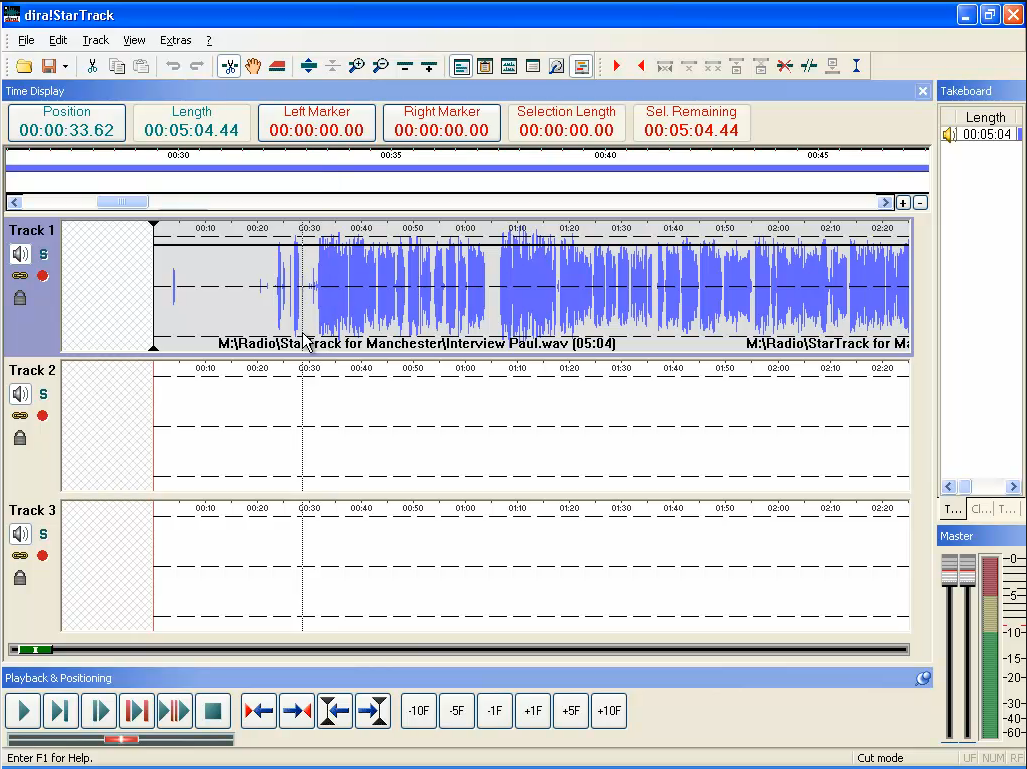
\includegraphics[width=0.8\textwidth]{figs/startrack.png}
\caption{The user interface for StarTrack.}
\label{fig:startrack}
\end{figure}

\paragraph{Modes}
There are three modes in which the StarTrack interface can operate. The default
-- `\textbf{edit mode}' -- is where audio clips can be cut and trimmed,
`\textbf{arrange mode}' is targeted towards moving clips around and
`\textbf{level mode}' is for editing level automation

The primary difference between the modes is the behaviour of the mouse. In
edit mode, clicking the left button sets the position of the cursor, the right
button allows clips to be moved, and dragging with the left button makes a
selection of audio. In arrange mode, the left button selects clips, dragging
moves them around and the middle button sets the position of the cursor. In
level mode, the mouse can be used to move, create and delete nodes in the level
automation.
% what does the right button do?

\paragraph{Playback}
The interface contains five play modes, which were chosen to cater for the most
common editing tasks. They are listed below with their keyboard shortcuts. The
default for $x$ is 2.

\begin{itemize}
  \item \texttt{[space]} Normal playback
  \item \texttt{[B]} Play $x$ seconds from cursor position - used to check
    intro before topping clip. \texttt{[Backspace]} operates in a similar way,
    but with a 5 second lead-up.
  \item \texttt{[V]} Play $x$ seconds up to cursor position - used to check
    outro before tailing clip
  \item \texttt{[N]} Play first and last $x$ seconds of selection - used to
    check selection before clipping
  \item \texttt{[M]} Play $x$ seconds before and $x$ seconds after selection -
    used to check selection before deleting\footnote{This method does not
      perform a crossfade so is not an accurate representation of how an edit
      would sound}
\end{itemize}

The speed of playback can be controlled using the \texttt{[$\uparrow$]} and
\texttt{[$\downarrow$]} buttons, which increases/decreases the rate at which
the audio samples are played (giving a `chipmunk' effect on speech). Pressing
\texttt{[$\downarrow$]} enough times reverses the direction of playback.

\paragraph{View}
The view can be manipluated in a number of ways. The height of the selected
track (vertical zoom) can be controlled with \texttt{[Page Up]}/\texttt{[Page
  Down]}, or by using the mouse to drag the boundaries between tracks. The time
span (horizontal zoom) can be controlled with \texttt{[+]}/\texttt{[-]}, or by
holding \texttt{[Ctrl]} and using the mouse scroll wheel. When some audio is
selected, pressing \texttt{[=]} fits the selection to the window (zoom to
selection).

Each clip has an associated colour and name, which are displayed using the
waveform and a label underneath. These can be changed by right-clicking the
clip and using the context menu.

Markers can be set using the \texttt{[\#]} key and they appear as a triangle at
the top of the track. Each marker has an associated colour and label, although
the label isn't visible. They can be edited by right-clicking on the marker.
Markers are affixed to the audio data, so they remain in place when clips are
copied or moved.

\paragraph{Navigation}
In addition to using the mouse to navigate (as described in the `modes'
section), navigation and selection is aided through the use of a number of
shortcuts:
\begin{itemize}
  \item \texttt{[$\leftarrow$]}/\texttt{[$\rightarrow$]} Move to the
    previous/next edit point or marker. Use with \texttt{[$\Uparrow$]} to move
    to beginning/end of selection.
  \item \texttt{[Home]/[End]} Select to start/end of clip. Use with
    \texttt{[Ctrl]} to move the cursor
  \item \texttt{[7]/[8]} Nudge/nibble the start of the selection left/right
  \item \texttt{[9]/[0]} Nudge/nibble the end of the selection left/right
  \item \texttt{[ / ]} Set in/out markers for selection while playing
\end{itemize}

\paragraph{Editing}

\verb$[\]$ splits a clip into two at the point of the cursor. A solid line
shows that the clip is not connected, and the two parts can be moved freely.

\texttt{[Delete]} removes a selection of audio from a clip and joins the two
remaining parts of the clip together with a crossfade. The edit is shown as a
dotted line with an empty triangle at the top, indicating that the two
remaining parts are connected and move together. The user can undo the edit at
a later stage by right-clicking the triangle and selecting `undo edit'.

\texttt{[w]} removes the selected audio, but separates the remaining two parts
into individual clips and leaves a gap in the middle.

Fade in/out operations must be done using the mouse. There is a triangle in the
top left/right corner of each clip which, when dragged, applies a fade in/out.
It can also be done by making a selection and using the context menu, which has
three curve options.

When clips overlap on a track, their output is played simultaneously. Any
crossfading between the two must be done manually by using level automation.

\paragraph{Levels}
By default, each clip displays a solid horizontal black line which represents a
0dB gain for that clip. It can be moved up and down with the mouse in edit
mode. Holding \texttt{[Ctrl]} changes the level only in the selected region and
holding \texttt{[$\Uparrow$]} affects all of the clips in that track.

Switching to level mode allows finer control using level automation. Nodes can
be created by dragging the first/last node in a clip, or holding
\texttt{[Ctrl]} while clicking on the black line. Nodes can be deleted by
holding \texttt{[Ctrl]} and clicking on an existing node.

\paragraph{Takeboard and clipboard}
The `takeboard' is a list displayed on the right of the interface which
contains a list of all raw audio recordings that are available. They can be
dragged and dropped onto a track.

The `clipboard' contains a list of clips. In this context, a `clip' is a copy
of an edit, which can be made by highlighting part of a track and pressing
\texttt{[C]}. The clip will include any level automation and can include parts
of multiple audio files and silences. In that respect, it can be considered to
be a mini EDL. Deleting a clip does not destroy any raw audio data.

The list of clips can be reordered, and by selecting multiple clips from the
list and dragging them onto a track, they will be inserted one after the other.
This functionality is useful for putting together a rough edit.  Pressing
\texttt{[P]} will preview the selected clip in a small preview window. The
preview only contains play, stop and scroll functionality, but audio can be
selected and dragged onto a track. Clips can be `bounced down' to an audio file
using the context menu.

\paragraph{Slips and chains}
When audio clips (or parts of clips) are removed\slash inserted\slash moved,
the clips to the right of the edit on that track are automatically moved to
fill/accomodate the edit. When multiple tracks are used, this can cause tracks
to fall out-of-sync with each other, but this can be fixed by using either
chaining or slipping.

Chaining is where multiple tracks are grouped together so that when audio is
removed\slash inserted\slash moved, all of the clips on the chained tracks move
together.  When audio is selected on a chained track, it is selected across all
of the chained tracks.

Slipping is similar to chaining but affects all tracks, not just those chained
together. StarTrack provides the option of `right slip', where clips on every
track to the right of the edit move together, or `left slip' where the clips to
the left of the edit move together. Both can be used at the same time, which
gives the effect of chaining all tracks.

Tracks can also be locked so that they are unaffected by actions in other
tracks. This is useful for content such as background music, which doesn't need
to be in sync.

\paragraph{Signal processing}
StarTrack includes support for VST audio effect plugins. A number of
VCS-branded plugins are supplied as standard, including ones for dynamics,
parametric EQ, graphic EQ and mixing. A simulated PPM meter is also available
for checking levels. However, the VST support in StarTrack is currently limited
to VST v2.0, can only support stereo signals and doesn't support channel
mapping. Parametric EQ can also be applied to clips individually through a menu
option.

\paragraph{Saving and bouncing down}
Projects can be saved either `without audio', where the audio data remains
stored in the dira! system, or `with audio', where the audio is copied onto the
local machine. BBC best practise stipulates that the audio should be stored on
dira! whenever possible in order to avoid data loss and to make the files
available to other staff members.

StarTrack performs a local background autosave every two minutes where projects
can be restored through a menu option. When a project is `bounced down' to an
audio file, only the tracks which are visible in the interface are included in
the mix. This can be useful for easily excluding tracks, but is usual behaviour
for a DAW, so could catch people out.
